\subsection{Appearance Editor}
\label{sec:sf-appearance}
\writer{Monica}

The Appearance Editor is a component that will allow the user to add visual information such as 3D objects and textures to the Petri net objects to be simulated. The connection between the appearance files and the Petri net objects will be done via the \textit{appearance labels} defined by the user in the Geometry editor (See section \ref{sec:sf-geometry}). 

Before using the Appearance Editor, the user has to \textit{create} a new or \textit{load} an existing appearance file he/she wants to edit.

\subsubsection{Functional Requirements}

\begin{enumerate}
\item The Appearance Editor \textbf{shall} allow the user to create new appearance objects, \textit{AObject}.
\item The Appearance Editor \textbf{shall} allow the user to input the name of an appearance label for an AObject.
\item It \textbf{would be nice} to allow the user to load a Geometry file in order to retrieve all the appearance labels.
\item The Appearance Editor \textbf{shall} allow the user to input the path of a predefined 3D object file for an  AObject.
\item The Appearance Editor \textbf{shall} allow the user to input the path of a predefined texture file for an AObject.
\item The Appearance Editor \textbf{shall} allow the user to save an Appearance file.
     
\end{enumerate}

\subsubsection{Use cases}

The features described above are shown in the following use case diagram Figure~\ref{fig:use-cases-appearance-editor}.

\begin{figure}[htp]
\begin{center}
  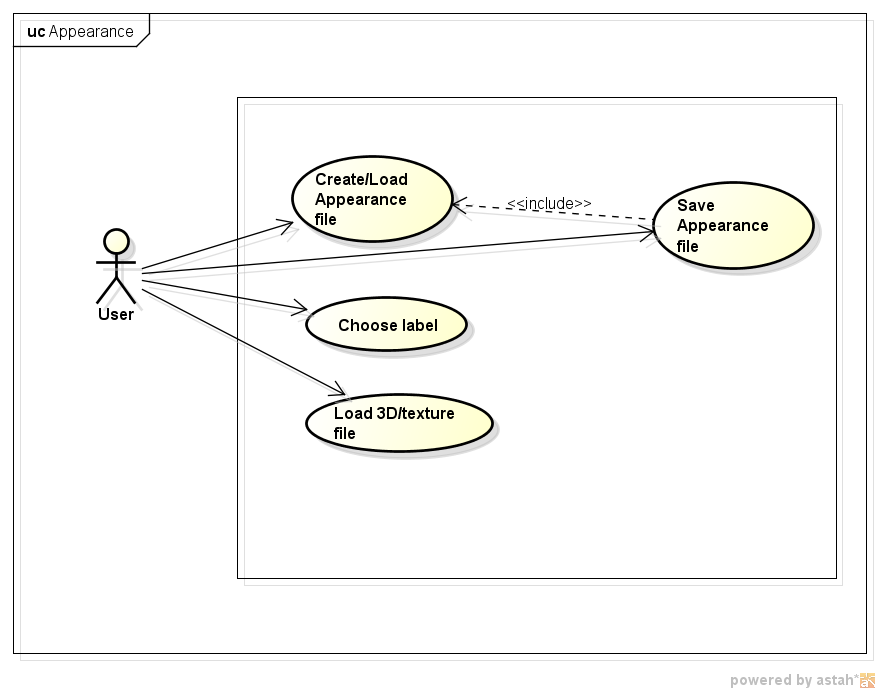
\includegraphics[width=0.5\textwidth]{image/uc-appearance.png}
  \caption{Use cases for the Appearance Editor}
  \label{fig:use-cases-appearance-editor}
\end{center}
\end{figure}

